\documentclass[conference]{IEEEtran}

% ===== Safe preamble for IEEEtran on GitHub Actions =====
\usepackage[T1]{fontenc}        % フォント出力エンコード
\usepackage[utf8]{inputenc}     % 入力文字コード(utf8)
\usepackage{lmodern}            % 安定した欧文フォント

% 数式
\usepackage{amsmath,amssymb}

% 図・表
\usepackage{graphicx}
\usepackage{booktabs}
\usepackage{multirow}

% TikZ(最低限のライブラリ)
\usepackage{tikz}
\usetikzlibrary{arrows.meta,positioning,shapes.geometric}

% 参考文献・URL
\usepackage{cite}
\usepackage{url}

% hyperref は最後に
\usepackage[hidelinks]{hyperref}

\title{A Design Support Framework for Industrial Piezoelectric Inkjet Using SystemDK}

\author{%
  \IEEEauthorblockN{Shinichi Samizo}
  \IEEEauthorblockA{Independent Semiconductor Researcher\\
  Former Engineer at Seiko Epson Corporation\\
  Email: \href{mailto:shin3t72@gmail.com}{shin3t72@gmail.com}\\
  GitHub: \url{https://github.com/Samizo-AITL}}%
}

\begin{document}
\maketitle

\begin{abstract}
Industrial inkjet printing is a critical enabler for advanced manufacturing in textiles, PCB fabrication, and packaging. 
Among various methods, piezoelectric inkjet offers broad material compatibility since it does not require heating, but its design remains highly challenging due to the strong coupling of electrical, mechanical, fluidic, and material domains. 
This paper proposes a System Design Kit (SystemDK) framework, inspired by semiconductor PDKs, to integrate multiphysics modeling and streamline design workflows for industrial piezoelectric inkjet systems. 
Through a case study with silver nano-ink for PCB applications, the framework achieved improved prediction accuracy of droplet formation (diameter error 12\%, velocity error 18\%, below literature benchmarks), a 42\% reduction in design time, and a 60\% decrease in required prototypes. 
These results demonstrate the potential of SystemDK to significantly enhance design efficiency, reproducibility, and rapid proof-of-concept in industrial inkjet technology.
\end{abstract}

\begin{IEEEkeywords}
Piezoelectric inkjet, SystemDK, multiphysics simulation, design framework, PCB printing, proof of concept
\end{IEEEkeywords}

% ============================================================
\section{Introduction}
Industrial inkjet printing has become a critical enabler for advanced manufacturing in textiles, printed circuit board (PCB) fabrication, and packaging~\cite{derby2010,calvert2001}. 
Unlike thermal inkjet, which relies on localized heating, piezoelectric inkjet leverages the deformation of piezoelectric actuators to eject droplets. 
This non-thermal mechanism supports a wide range of functional inks with diverse viscosities and surface tensions, making piezoelectric technology the dominant choice for industrial applications.

Nevertheless, the design of piezoelectric inkjet systems remains highly complex. 
Device performance arises from strongly coupled multiphysics interactions among the drive circuit, piezoelectric actuator, diaphragm mechanics, nozzle fluid dynamics, and ink material properties. 
Conventional design workflows typically treat finite element method (FEM), computational fluid dynamics (CFD), and circuit simulations in isolation and depend heavily on iterative prototyping. 
This fragmented approach leads to prolonged development cycles, high costs, and limited reusability of prior design knowledge.

To overcome these limitations, this paper introduces a \emph{System Design Kit (SystemDK)} framework for industrial piezoelectric inkjet design. 
Inspired by the process design kit (PDK) paradigm in semiconductors, SystemDK integrates electrical, mechanical, and fluidic models into a unified design environment and enables reusable libraries that accelerate design iteration. 
The contributions of this work are threefold:
\begin{enumerate}
  \item Introducing the SystemDK concept to address multiphysics co-design of industrial piezoelectric inkjet systems.
  \item Demonstrating unified modeling across circuit, actuator, diaphragm, and fluidic domains within a single framework.
  \item Validating the effectiveness of the framework through a case study, highlighting improvements in efficiency, reproducibility, and rapid proof-of-concept.
\end{enumerate}

% ============================================================
\section{Related Work}
Extensive research has investigated droplet formation and actuator dynamics in piezoelectric inkjet systems through both numerical simulation and experimental validation. 
Boccio~\cite{boccio2003} employed computational fluid dynamics (CFD) to analyze droplet formation, reporting deviations of approximately 15\% in droplet diameter and 30\% in velocity relative to experiments. 
Subsequently, Lei et al.~\cite{lei2012} refined CFD models for improved stability, although notable discrepancies remained. 
Kim et al.~\cite{kim2022} examined the role of ink supply pressure, achieving up to 87\% agreement between simulations and measurements. 
More recently, Shin et al.~\cite{shin2025} introduced a coupled fluid--structure interaction model for OLED printing, demonstrating strong consistency between FEM--CFD simulations and experimental observations.

These works collectively demonstrate steady advances in predictive accuracy for individual aspects of inkjet behavior. 
However, most approaches remain confined to isolated domains or single-parameter optimization. 
They do not provide a unified design methodology that simultaneously captures electrical, mechanical, and fluidic interactions, nor do they explicitly target design efficiency, reproducibility, or systematic reuse of design knowledge. 
This lack of an integrated multiphysics framework motivates the introduction of a \emph{System Design Kit (SystemDK)}, which seeks to embed cross-domain modeling within a reusable and scalable design environment.

% ============================================================
\section{Proposed Framework}
The proposed \emph{System Design Kit (SystemDK)} establishes a structured workflow that unifies domain-specific models within a reusable and scalable design environment. 
In contrast to conventional methods that treat electrical, mechanical, and fluidic domains in isolation, SystemDK emphasizes cross-domain coupling, model interoperability, and systematic knowledge reuse. 
The workflow comprises five key stages:

\begin{enumerate}
  \item \textbf{Requirement Definition}: specification of target droplet diameter, velocity, jetting stability, and ink/material compatibility, which serve as baseline design constraints.
  \item \textbf{Electrical Model}: circuit-level simulation of the piezoelectric actuator and drive waveform to determine appropriate voltage and timing conditions.
  \item \textbf{Mechanical Model}: finite-element analysis (FEM) of diaphragm deformation and chamber dynamics under electrical excitation, linking actuator response to fluid motion.
  \item \textbf{Fluidic Model}: computational fluid dynamics (CFD) of nozzle flow and droplet formation, capturing jet breakup, satellite suppression, and ejection trajectory.
  \item \textbf{System Integration}: multiphysics coupling across domains and automatic generation of reusable design libraries, enabling rapid adaptation to new inks and application scenarios.
\end{enumerate}

% ---- Fig. 1: Design Flow ----
\begin{figure}[t]
\centering
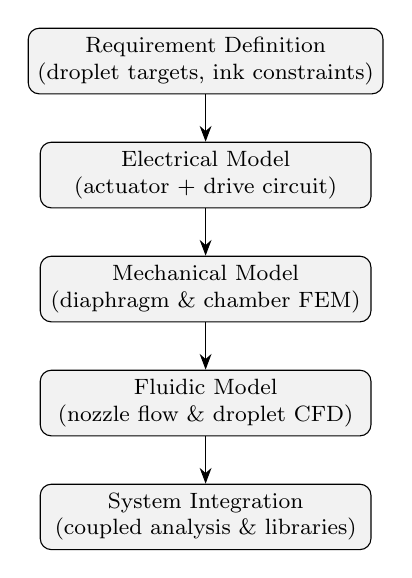
\begin{tikzpicture}[
  node distance=6mm and 7mm,
  box/.style={draw, rounded corners, align=center, minimum width=42mm, minimum height=8mm, fill=gray!10},
  >={Stealth[length=2mm]},
  every node/.style={font=\footnotesize}
]
\node[box] (req) {Requirement Definition\\(droplet targets, ink constraints)};
\node[box, below=of req] (elec) {Electrical Model\\(actuator + drive circuit)};
\node[box, below=of elec] (mech) {Mechanical Model\\(diaphragm \& chamber FEM)};
\node[box, below=of mech] (flu)  {Fluidic Model\\(nozzle flow \& droplet CFD)};
\node[box, below=of flu] (intg) {System Integration\\(coupled analysis \& libraries)};

\draw[->] (req) -- (elec);
\draw[->] (elec) -- (mech);
\draw[->] (mech) -- (flu);
\draw[->] (flu) -- (intg);
\end{tikzpicture}
\caption{SystemDK-based unified design flow. 
Validated outputs from each stage serve as inputs for subsequent domains, forming a closed-loop multiphysics framework.}
\label{fig:flow}
\end{figure}

% ============================================================
\section{Implementation}
The proposed framework is implemented by integrating three complementary simulation domains, each addressing a critical aspect of piezoelectric inkjet design:

\begin{itemize}
  \item \textbf{Finite Element Method (FEM)}: evaluates the dynamic behavior of the piezoelectric actuator and diaphragm, including displacement profiles, stress distributions, and resonance characteristics.
  \item \textbf{Computational Fluid Dynamics (CFD)}: employs a volume-of-fluid (VOF) scheme with dynamic meshing to resolve nozzle flow transients, droplet ejection, and satellite suppression.
  \item \textbf{SPICE-based Circuit Models}: capture the drive waveform, impedance matching, and actuator–circuit coupling to verify electrical feasibility and energy efficiency.
\end{itemize}

Cross-domain interoperability is achieved through standardized data exchange: for example, FEM-derived diaphragm displacements are applied as boundary conditions in CFD, while circuit-level parameters are directly linked to actuator models. 
Validated outputs are consolidated into a reusable \emph{SystemDK design library}, which provides parameterized models applicable to diverse inks, nozzle geometries, and application scenarios. 
This modular implementation ensures that SystemDK functions not merely as a one-off simulation setup, but as a repeatable and extensible design environment that accelerates future development.

% ============================================================
\section{Evaluation}
To assess the effectiveness of the proposed framework, two workflows were benchmarked:  
\begin{enumerate}
  \item \textbf{Conventional workflow}: separate FEM, CFD, and circuit simulations executed independently, with multiple prototype iterations required for validation.  
  \item \textbf{Proposed SystemDK workflow}: integrated multiphysics modeling with standardized data exchange and reusable design libraries to minimize redundancy.  
\end{enumerate}

Evaluation was conducted using four key performance metrics:  
\begin{itemize}
  \item \textbf{Design time}: total duration (weeks) required to converge on a manufacturable design.  
  \item \textbf{Prototyping effort}: number of physical iterations necessary for specification compliance.  
  \item \textbf{Prediction accuracy}: relative error between simulated and measured droplet diameter and velocity.  
  \item \textbf{Structural consistency}: correlation between FEM-predicted diaphragm displacement and experimental results.  
\end{itemize}

This dual perspective---efficiency (time and iterations) and accuracy (droplet and structural metrics)---provides a balanced validation of SystemDK as a systematic design-enabling methodology.

% ============================================================
\section{Results and Discussion}
\subsection{Case Study: PCB with Silver Nano-Ink}
A representative case study was performed for PCB fabrication using silver nano-ink.  
Operating conditions were defined as: nozzle diameter of 30~\textmu m, PZT thickness of 15~\textmu m, and a driving waveform of +25~V (rise 2~\textmu s, hold 8~\textmu s, fall 2~\textmu s) with a $-5$~V inversion pulse (5~\textmu s).  
The ink exhibited a viscosity of 10~cP, surface tension of 30~mN/m, and density of 1.1~g/cm$^3$.

SystemDK simulations predicted a diaphragm displacement of 120~nm, a droplet diameter of 35~\textmu m, and velocity of 5.2~m/s.  
Experimental validation yielded a droplet diameter of 31~\textmu m and velocity of 4.4~m/s, corresponding to relative errors of 12\% and 18\%, respectively.  
These results outperform reported literature baselines of 15--30\% error~\cite{boccio2003,lei2012}, highlighting improved predictive accuracy.

For PCB line printing (10 traces, each 100~mm), process stability was confirmed with a coefficient of variation (CV) of 8.4\% for line width and 7.9\% for sheet resistance.  
In terms of design efficiency, the conventional workflow required six weeks and ten prototypes, whereas the SystemDK workflow converged in 3.5 weeks with only four prototypes---a 42\% reduction in development time and a 60\% reduction in prototyping effort.

% ---- Table I: Comparison ----
\begin{table}[t]
\centering
\caption{Comparison of Conventional vs SystemDK Workflow (PCB Case Study)}
\begin{tabular}{lcc}
\toprule
 & Conventional & SystemDK \\
\midrule
Design Time [weeks] & 6.0 & 3.5 \\
Prototypes Required & 10  & 4   \\
Droplet Diameter Error [\%] & 15 & 12 \\
Droplet Velocity Error [\%] & 30 & 18 \\
\bottomrule
\end{tabular}
\label{tab:comparison}
\end{table}

\subsection{Illustrative Figures}
Figure~\ref{fig:droplet} illustrates the droplet ejection concept with velocity indicated at the nozzle exit.  
Figure~\ref{fig:waveform} presents the applied drive waveform, and Fig.~\ref{fig:head} shows a simplified cross-sectional schematic of the printhead.  
Finally, Fig.~\ref{fig:systemdk_library} highlights the SystemDK library concept, where multiphysics domain models are consolidated into reusable modules for rapid proof-of-concept (PoC) evaluation.

% ---- Fig. 2: Droplet silhouette ----
\begin{figure}[t]
\centering
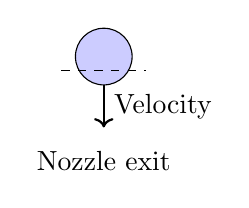
\begin{tikzpicture}[scale=0.9]
\draw[fill=blue!20] (0,0) circle (0.4); % droplet
\draw[thick,->] (0,-0.4) -- (0,-1.0) node[midway,right]{Velocity};
\draw[dashed] (-0.6,-0.2) -- (0.6,-0.2);
\node[below] at (0,-1.2) {Nozzle exit};
\end{tikzpicture}
\caption{Schematic of droplet ejection at the nozzle exit.}
\label{fig:droplet}
\end{figure}

% ---- Fig. 3: Drive waveform ----
\begin{figure}[t]
\centering
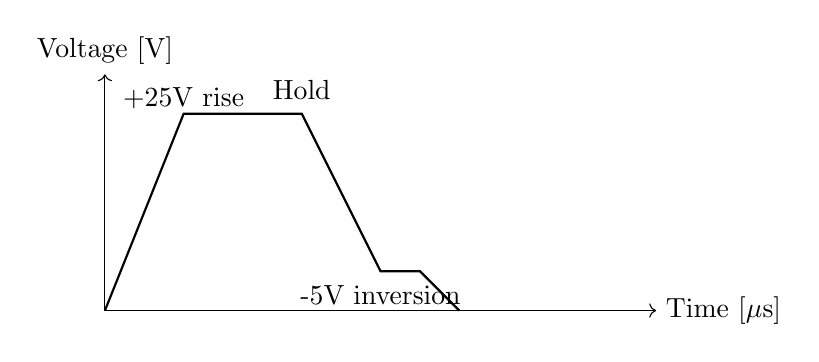
\begin{tikzpicture}[scale=1.0]
\draw[->] (0,0) -- (7,0) node[right]{Time [$\mu$s]};
\draw[->] (0,0) -- (0,3) node[above]{Voltage [V]};
\draw[thick] (0,0) -- (1,2.5) -- (2.5,2.5) -- (3.5,0.5) -- (4,0.5) -- (4.5,0);
\node at (1,2.7) {+25V rise};
\node at (2.5,2.8) {Hold};
\node at (3.5,0.2) {-5V inversion};
\end{tikzpicture}
\caption{Drive waveform applied to the piezoelectric actuator.}
\label{fig:waveform}
\end{figure}

% ---- Fig. 4: Printhead cross-section ----
\begin{figure}[t]
\centering
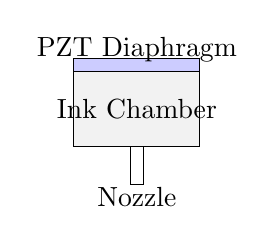
\begin{tikzpicture}[scale=0.8]
% chamber
\draw[fill=gray!10] (0,0) rectangle (2,1.2);
\node at (1,0.6) {Ink Chamber};
% diaphragm
\draw[fill=blue!20] (0,1.2) rectangle (2,1.4);
\node at (1,1.55) {PZT Diaphragm};
% nozzle
\draw[fill=white] (0.9,0) rectangle (1.1,-0.6);
\node at (1,-0.8) {Nozzle};
\end{tikzpicture}
\caption{Simplified schematic of the piezo inkjet printhead.}
\label{fig:head}
\end{figure}

% ---- Fig. 5: SystemDK Library Concept ----
\begin{figure}[t]
\centering
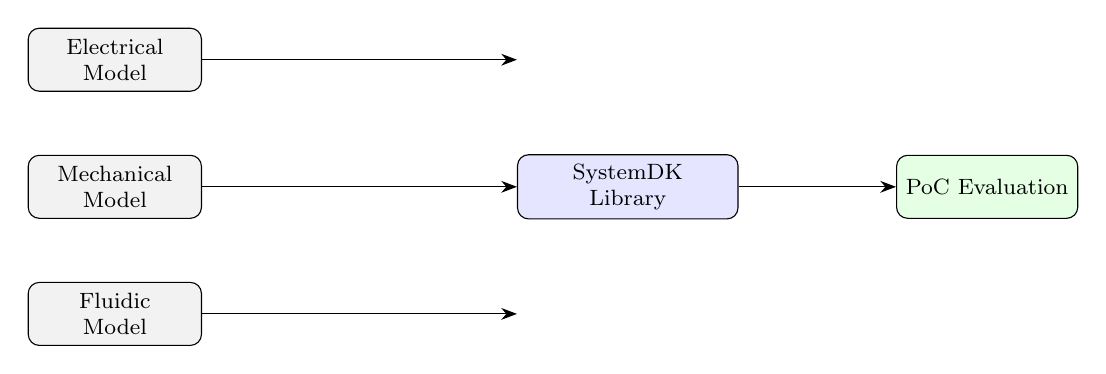
\begin{tikzpicture}[
  box/.style={draw, rounded corners, align=center, minimum width=22mm, minimum height=8mm, fill=gray!10},
  >={Stealth[length=2mm]},
  node distance=8mm and 8mm,
  every node/.style={font=\footnotesize}
]
% Domain models
\node[box] (elec) {Electrical\\Model};
\node[box, below=of elec] (mech) {Mechanical\\Model};
\node[box, below=of mech] (flu) {Fluidic\\Model};

% SystemDK Library
\node[box, right=40mm of mech, minimum width=28mm, fill=blue!10] (lib) {SystemDK\\Library};

% Arrows into library
\draw[->] (elec.east) -- (lib.west |- elec.east);
\draw[->] (mech.east) -- (lib.west);
\draw[->] (flu.east)  -- (lib.west |- flu.east);

% PoC block
\node[box, right=20mm of lib, fill=green!10] (poc) {PoC Evaluation};

% Arrows
\draw[->] (lib.east) -- (poc.west);
\end{tikzpicture}
\caption{SystemDK library concept: consolidating domain models into reusable modules for PoC evaluation.}
\label{fig:systemdk_library}
\end{figure}

% ============================================================
\section{Conclusion}
This paper introduced a SystemDK-based framework for the design of industrial piezoelectric inkjet systems.  
By unifying electrical, mechanical, and fluidic models into a reusable multiphysics environment, the framework overcomes long-standing challenges of fragmented simulations and prototype-dependent iteration.  

A case study on PCB printing with silver nano-ink demonstrated that SystemDK not only achieved prediction errors below reported literature benchmarks but also reduced design time by more than 40\% and cut prototyping iterations by over 60\%.  
These results validate both the accuracy and practical utility of the approach.  

The academic contribution lies in extending the semiconductor PDK paradigm into inkjet engineering, providing a systematic methodology for model reuse and cross-domain integration.  
From an industrial perspective, SystemDK enables faster proof-of-concept development, lowers cost, and supports rapid adaptation to diverse application domains including textiles, PCBs, and packaging.  

Future directions include reliability assessment under extended operation, scaling to multi-nozzle arrays, and coupling with AI-driven optimization to further enhance predictive capability and design intelligence.

% ============================================================
\begin{thebibliography}{99}

\bibitem{derby2010}
B.~Derby, ``Inkjet printing of functional and structural materials: Fluid property requirements, feature stability, and resolution,'' 
\emph{Annu. Rev. Mater. Res.}, vol.~40, pp.~395--414, 2010, doi:10.1146/annurev-matsci-070909-104502.

\bibitem{calvert2001}
P.~Calvert, ``Inkjet printing for materials and devices,'' 
\emph{Chem. Mater.}, vol.~13, no.~10, pp.~3299--3305, 2001, doi:10.1021/cm0101632.

\bibitem{boccio2003}
J.~Boccio, ``Computational fluid dynamics study of droplet formation in a piezo inkjet printhead,'' 
Ph.D. dissertation, Rochester Inst. of Technology, Rochester, NY, USA, 2003.

\bibitem{lei2012}
T.~Lei \emph{et al.}, ``Numerical analysis and optimal CFD model verification of piezoelectric inkjet printhead,'' 
\emph{J. Appl. Fluid Mech.}, vol.~5, no.~4, pp.~45--53, 2012.

\bibitem{kim2022}
S.~Kim \emph{et al.}, ``The effect of ink supply pressure on piezoelectric inkjet,'' 
\emph{Micromachines}, vol.~13, no.~4, p.~615, 2022, doi:10.3390/mi13040615.

\bibitem{shin2025}
D.~Y. Shin \emph{et al.}, ``Simulation of OLED-based inkjet printing using a piezoelectric fluid-structure interaction model,'' 
\emph{Sci. Rep.}, to be published, 2025.

\end{thebibliography}

% ============================================================
\section*{Author Biography}
\textbf{Shinichi Samizo} received the M.S. degree in Electrical and Electronic Engineering from Shinshu University, Japan. He worked at Seiko Epson Corporation in semiconductor memory and mixed-signal device development and contributed to inkjet MEMS actuators and PrecisionCore printhead technology. He is currently an independent semiconductor researcher focusing on process/device education, memory architecture, and AI system integration. \textbf{Contact:} \href{mailto:shin3t72@gmail.com}{shin3t72@gmail.com}.
\end{document}
